\documentclass[11pt,a4paper,fontset=fandol]{ctexart}

\usepackage{geometry}
\geometry{a4paper, left=2.2cm, right=2.2cm, top=2.2cm, bottom=2.2cm, headheight=14pt}
\usepackage{setspace}
\linespread{1.05}
\usepackage{indentfirst}
\setlength{\parindent}{2em}
\emergencystretch=2em

\usepackage{xcolor}
\definecolor{themecolor}{RGB}{40,90,140}
\definecolor{codebg}{RGB}{248,248,245}

\usepackage{graphicx}
\graphicspath{{results/}}
\usepackage{amsmath}
\usepackage{booktabs}
\usepackage{caption}
\captionsetup{font=small,labelfont={bf,color=themecolor}}
\usepackage{subcaption}
\usepackage{float}
\usepackage{array}
\usepackage{verbatim}
\usepackage{hyperref}
\hypersetup{colorlinks=true, linkcolor=themecolor, citecolor=themecolor, urlcolor=themecolor!70!black}

\usepackage{titlesec}
\titleformat{\section}{\color{themecolor}\bfseries\fontsize{13}{16}\selectfont}{\thesection}{0.6em}{}
\titlespacing*{\section}{0pt}{0.9em}{0.35em}
\titleformat{\subsection}{\color{themecolor!85!black}\bfseries\fontsize{11.5}{14}\selectfont}{\thesubsection}{0.6em}{}
\titlespacing*{\subsection}{0pt}{0.55em}{0.15em}

\usepackage{fancyhdr}
\pagestyle{fancy}
\fancyhf{}
\renewcommand{\headrulewidth}{0.4pt}
\lhead{\small\color{black!55} 地图构建实验报告}
\rhead{\small\color{black!55} 人工智能 2302}
\cfoot{\small\color{black!55}\thepage}

\fancypagestyle{plain}{
  \fancyhf{}
  \renewcommand{\headrulewidth}{0pt}
  \cfoot{\small\color{black!55}\thepage}
}

\usepackage{mdframed}
\BeforeBeginEnvironment{verbatim}{
  \begin{mdframed}[
    backgroundcolor=codebg,
    linecolor=themecolor!30,
    linewidth=0.5pt,
    innerleftmargin=10pt,
    innerrightmargin=8pt,
    innertopmargin=6pt,
    innerbottommargin=4pt,
    skipabove=8pt,
    skipbelow=8pt,
    roundcorner=2pt,
  ]
}
\AfterEndEnvironment{verbatim}{\end{mdframed}}

\setCJKmonofont{Arial Unicode MS}

\title{\bfseries 地图构建实验报告}
\author{人工智能2302 \quad 蒋梓轩\\
人工智能2302 \quad 汪翌秦\\
人工智能2302 \quad 孙靖淞}
\date{2026 年 5 月 29 日}

\begin{document}

\maketitle

\section{实验目的}

本次实验围绕移动机器人二维栅格地图构建展开。实验在 Gazebo 仿真环境中加载带激光雷达的小车模型，启动 \verb|gmapping| 建图节点，通过键盘控制小车在场景中运动，使激光扫描数据和里程计信息共同生成环境占据栅格地图；同时在实车场景中整理 \verb|hector_mapping|、雷达、静态 TF 和底盘启动配置，为后续 AMCL 定位与路径规划提供静态地图基础。

通过实验需要掌握三点：第一，理解 \verb|/scan|、\verb|/tf|、\verb|/odom| 和 \verb|/map| 在 SLAM 建图中的作用；第二，理解 RViz 与 Gazebo 在仿真和可视化中的分工；第三，掌握使用 \verb|map_server| 保存 \verb|nav.pgm| 与 \verb|nav.yaml| 的流程。

\section{实验原理}

二维建图的核心是把激光雷达扫描和机器人位姿估计融合为占据栅格地图。对 \verb|gmapping| 来说，输入主要是激光雷达 \verb|/scan| 与 \verb|odom -> base_footprint| 坐标变换，输出是 \verb|map| 坐标系下的栅格地图；对 \verb|hector_mapping| 来说，算法更依赖高频激光扫描匹配，因此在里程计质量有限的实车场景中更容易快速建立可用地图。

\begin{table}[H]
  \centering
  \caption{建图实验关键数据流}
  \begin{tabular}{lll}
    \toprule
    数据或节点 & 作用 & 实验配置文件 \\
    \midrule
    \verb|/scan| & 提供障碍物距离观测 & \verb|my_lidar.launch| \\
    \verb|/tf| & 提供雷达、底盘、里程计坐标关系 & \verb|static_tf.launch| \\
    \verb|slam_gmapping| & 仿真环境中构建栅格地图 & \verb|slam_gmapping.launch| \\
    \verb|hector_mapping| & 实车环境中进行激光匹配建图 & \verb|slam_hector.launch| \\
    \verb|map_saver| & 保存 \verb|nav.pgm| 与 \verb|nav.yaml| & 命令行工具 \\
    \bottomrule
  \end{tabular}
\end{table}

\section{实验步骤与结果分析}

\subsection{仿真环境加载与建图}

实验首先启动 Gazebo，加载机器人模型和室内障碍物环境；随后启动 \verb|slam_gmapping.launch|，并通过键盘遥控小车在环境中移动。图 \ref{fig:lab3-process} 左图显示仿真环境已正确加载，机器人位于包含墙体、圆柱和方块障碍物的场景中；右图显示 RViz 中逐步生成的栅格地图，白色区域表示可通行空间，黑色区域表示障碍物边界。

\begin{figure}[H]
  \centering
  \begin{subfigure}{0.49\linewidth}
    \centering
    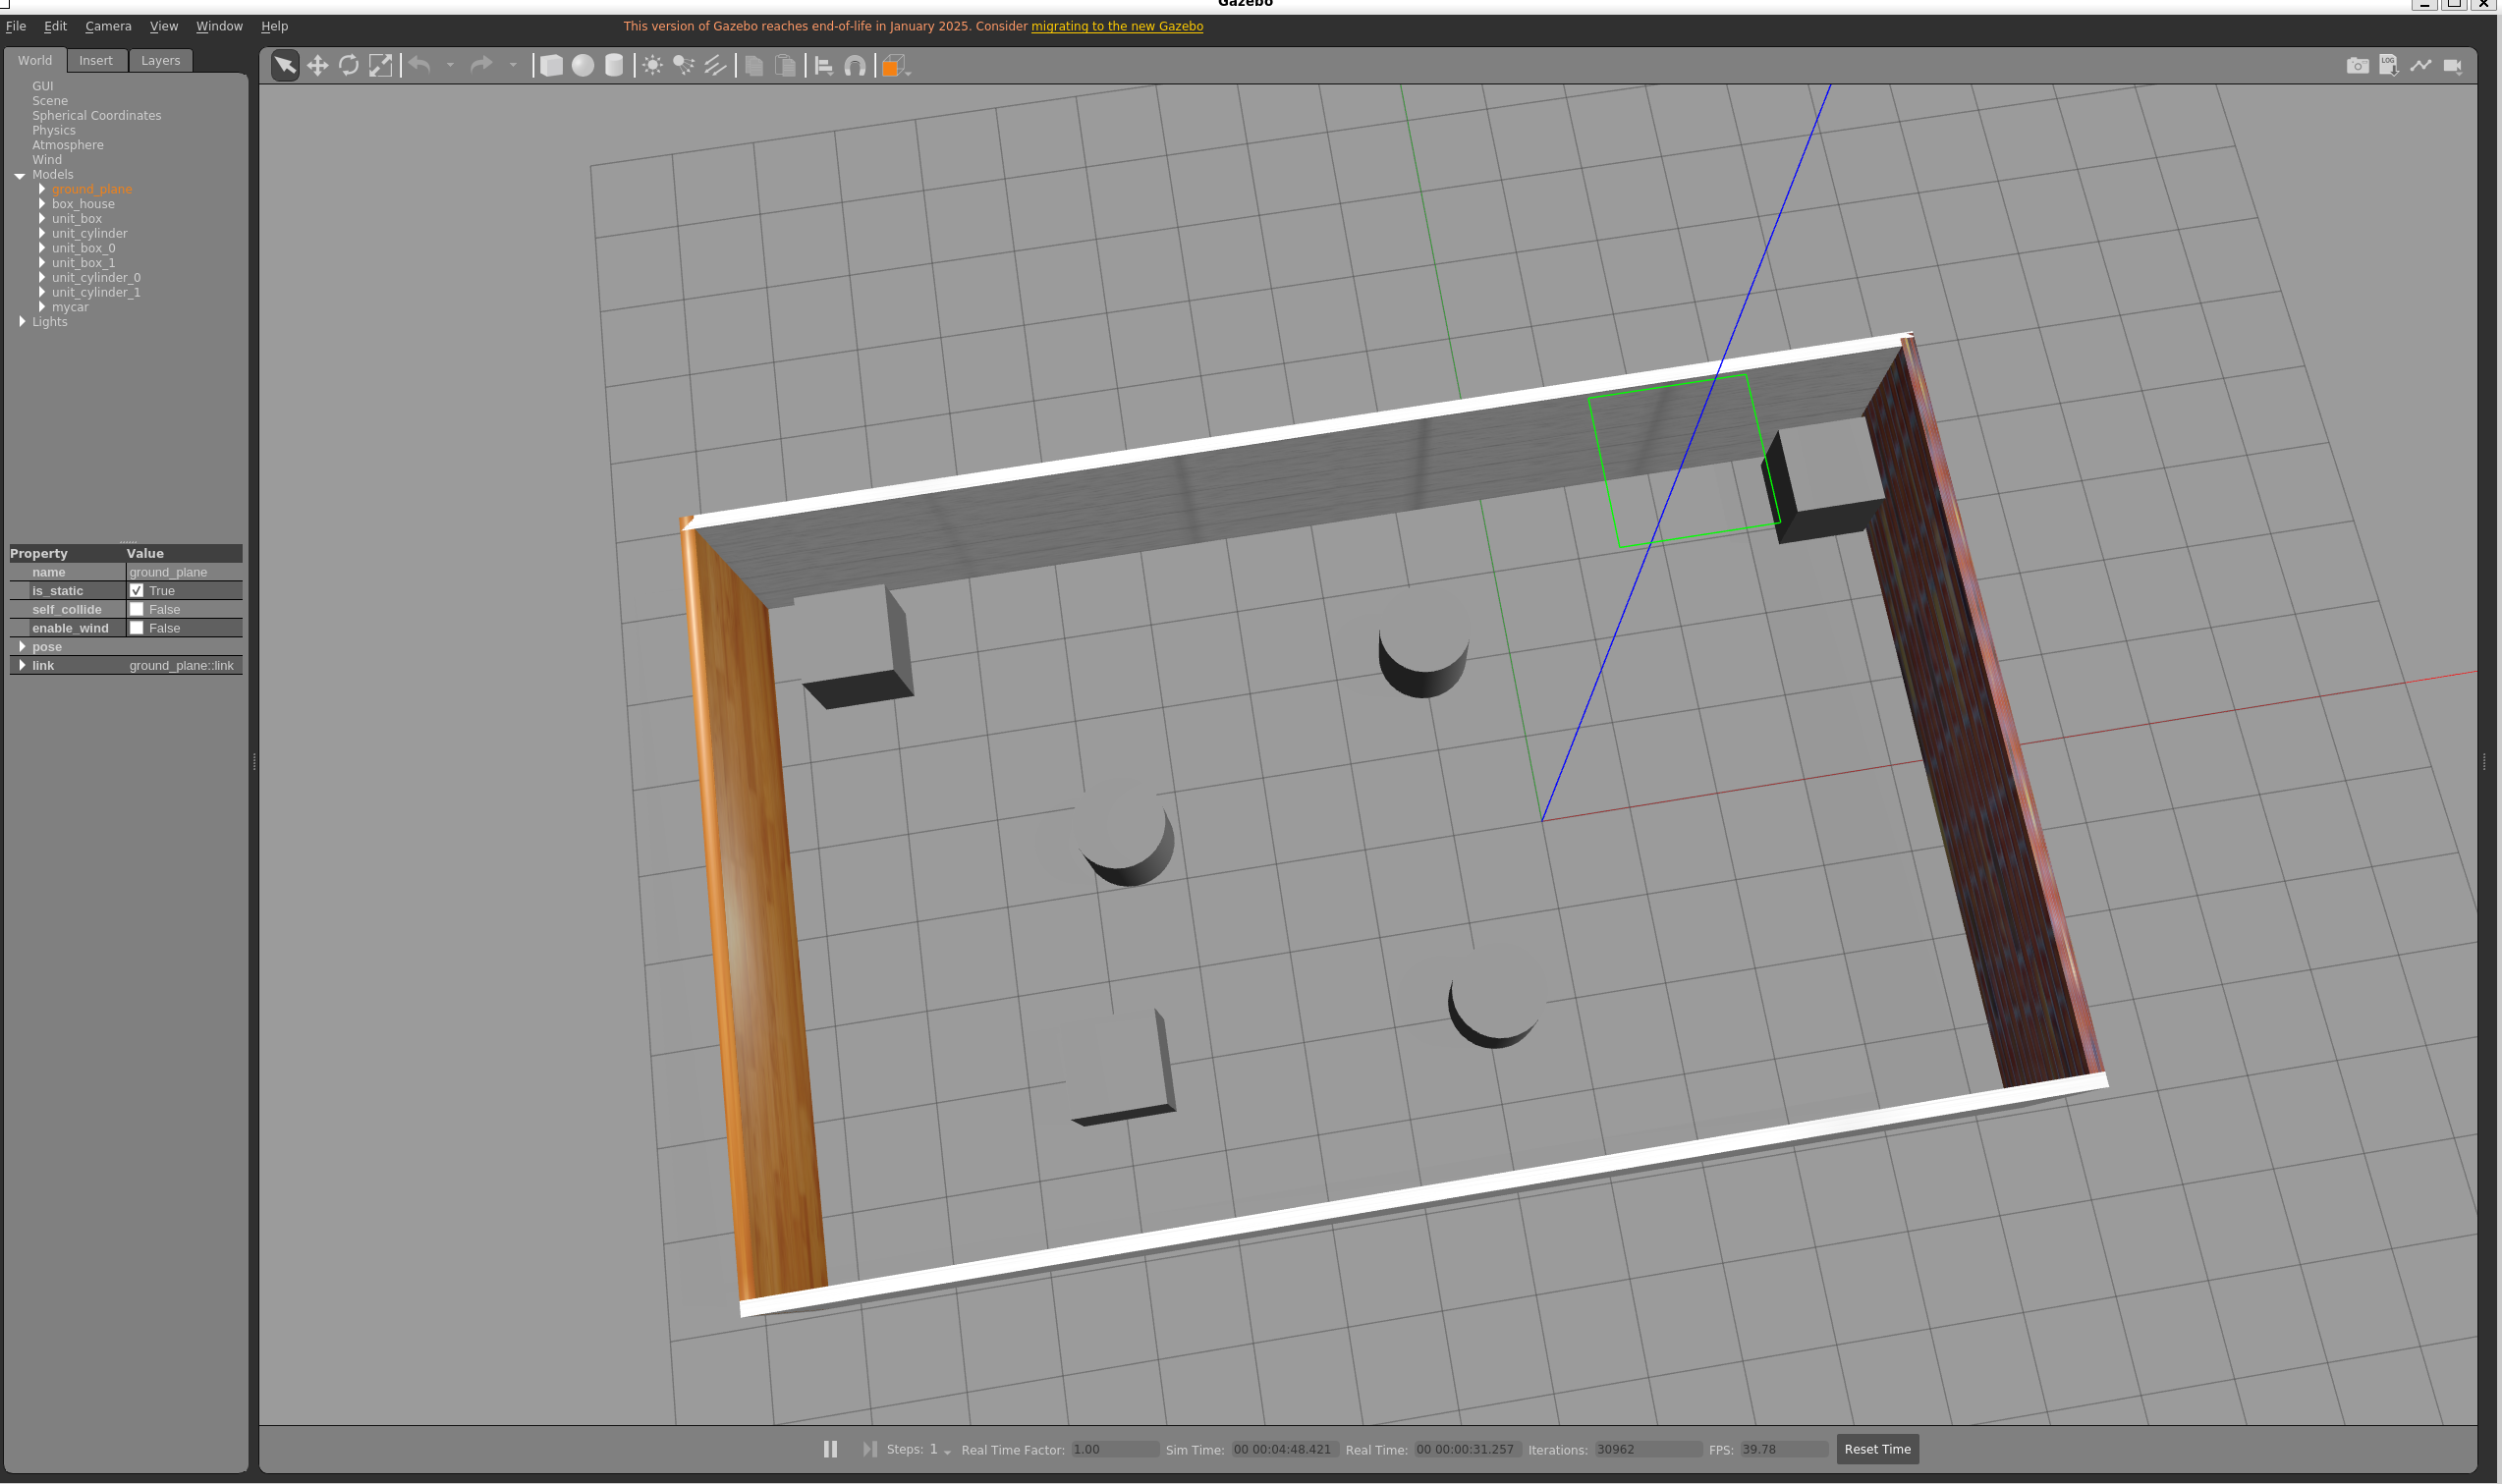
\includegraphics[width=\linewidth]{lab3_gazebo.png}
    \caption{Gazebo 仿真环境}
  \end{subfigure}
  \hfill
  \begin{subfigure}{0.49\linewidth}
    \centering
    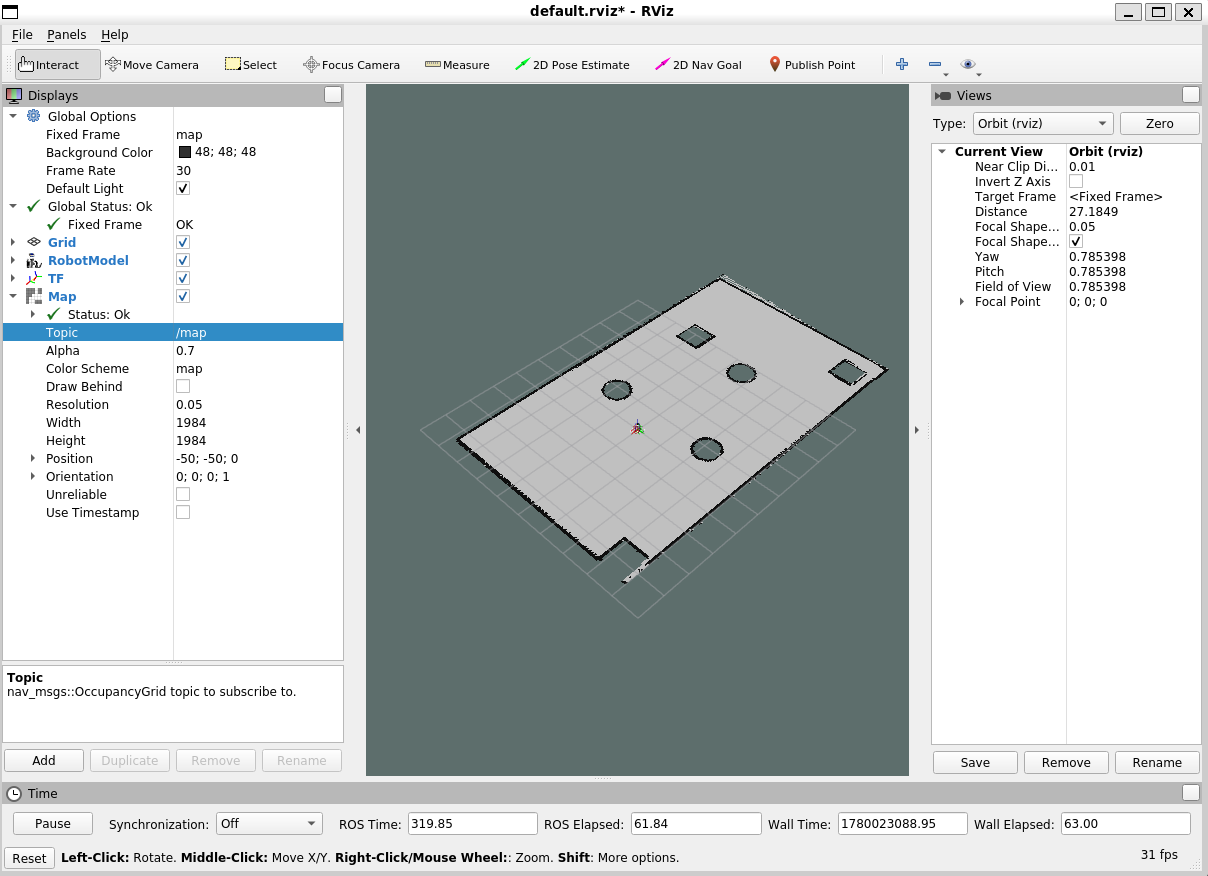
\includegraphics[width=\linewidth]{lab3_rviz_map.png}
    \caption{RViz 栅格地图结果}
  \end{subfigure}
  \caption{实验 3 地图构建过程与结果。}
  \label{fig:lab3-process}
\end{figure}

\subsection{地图保存与配置整理}

建图完成后，在 \verb|ebot_bringup/maps| 下使用 \verb|map_server| 保存地图：

\begin{verbatim}
rosrun map_server map_saver -f nav
\end{verbatim}

保存结果包括 \verb|nav.pgm| 和 \verb|nav.yaml|。其中 \verb|nav.pgm| 记录占据栅格图像，\verb|nav.yaml| 记录地图分辨率、原点、占据阈值等元数据。本次整理后的地图分辨率为 \verb|0.05 m/cell|，并继续作为实验 4 定位和实验 5 路径规划的静态地图输入。

\subsection{结果分析}

从 RViz 结果可以看到，主要障碍物边界已经被扫描并写入栅格地图。地图中局部边缘仍存在少量离散噪声，主要原因是遥控覆盖路径、激光扫描角度和 TF 标定误差都会影响栅格更新。为保证后续定位稳定，实验保存了较干净的 \verb|nav.pgm|/\verb|nav.yaml|，并将静态 TF 发布集中到 \verb|static_tf.launch|，减少重复发布或坐标链断裂导致的问题。

\section{结论与问题讨论}

本实验完成了从仿真环境加载、SLAM 节点启动、遥控扫描到地图保存的完整流程。实验结果表明，\verb|gmapping| 能够在仿真环境中利用里程计和激光雷达构建可用的二维栅格地图；实车配置中使用 \verb|hector_mapping| 更适合里程计不稳定或需要依赖激光匹配的场景。最终生成的 \verb|nav.pgm| 和 \verb|nav.yaml| 已满足后续 AMCL 定位与导航规划的输入要求。

\textbf{URDF、RViz、Gazebo 的作用。}
URDF 描述机器人模型结构和坐标关系；Gazebo 负责物理仿真、传感器仿真和环境交互；RViz 负责显示 ROS 话题、TF、地图和模型。Gazebo 更接近“运行世界”，RViz 更接近“观察数据”。

\textbf{雷达静态 TF 标定错误的影响。}
如果 \verb|base_footprint| 到雷达坐标系的平移或旋转错误，扫描点会被投影到错误位置，地图可能出现墙体偏移、障碍物重影、走廊弯曲或局部闭合错误，后续定位也会受到影响。

\textbf{Hector 与 Gmapping 的区别。}
\verb|gmapping| 通常依赖里程计和激光数据，适合仿真或里程计较可靠的移动平台；\verb|hector_mapping| 更依赖激光扫描匹配，对高频雷达友好，在缺少稳定轮式里程计时仍可建图。两者都会围绕 \verb|map|、\verb|odom|、\verb|base_footprint| 和雷达坐标系组织 TF，只是位姿估计来源不同。

\end{document}
